\chapter{Background and Existing Approaches}

\section{Introduction to Electrochemistry}

Electrochemistry is a process for determining the compounds in a solution. This is accomplished by causing reduction or oxidation within the solution by raising or lowering the potential near some electrode surfaces and measuring the amount of current that is generated.

Specifically, three electrodes (reference, auxiliary, working) are placed into a solution with an electroactive analyte. The potential difference between the electrodes is raised which creates a potential gradient at both electrode-solution interfaces, but a zero potential gradient in the bulk solution between the electrodes (Figure \ref{kissinger-6-5}). The field strength typically becomes zero at less than $10^{-6}\mathrm{m}$ from the surface of the electrode \cite{kissinger1996fca}. When the electroactive analyte nears an electrode, if the potential is high enough, an electron will find favorable conditions in the analyte and transfer from the surface of the electrode to the analyte. At this point there is a concentration gradient between the new, reduced, analyte and the original. The reduced analyte begins to diffuse into the bulk solution, causing more reductions to occur. This happens continuously and at an exponentially decreasing rate until all of the analyte has been reduced. The continuing transfer of electrons causes current to flow. A similar response called oxidation occurs if the potential is lowered and the electron transfers back to the electrode from the analyte. The potential is kept constant by the potentiostat (a device which performs these operations), which measures the current needed to keep the potential constant (Figure \ref{kissinger-6-4}).

\begin{figure}
	\centering
	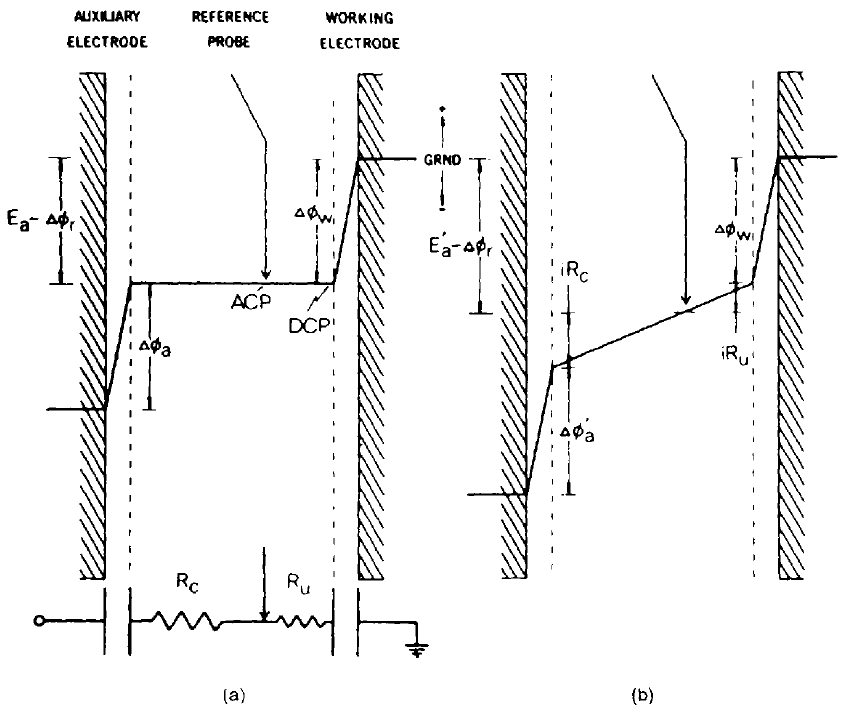
\includegraphics[width=0.5\linewidth]{figures/kissinger-6-5.png}
	\caption[Schematic representation of potential gradients in a three-electrode cell]{Schematic representation of potential gradients in a three-electrode cell: (a) $i = 0$; (b) $i \ne 0$. This is Figure 6.5 from \cite{kissinger1996iai}.}
	\label{kissinger-6-5}
\end{figure}

\begin{figure}
	\centering
	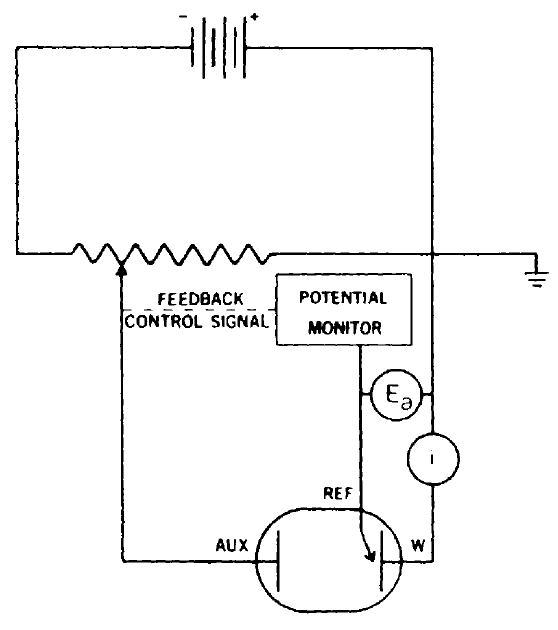
\includegraphics[width=0.5\linewidth]{figures/kissinger-6-4.png}
	\caption[Schematic representation of a primitive three-electrode controlled-potential apparatus]{Schematic representation of a primitive three-electrode controlled-potential apparatus. This is Figure 6.4 from \cite{kissinger1996iai}.}
	\label{kissinger-6-4}
\end{figure}

One technique is amperometry, where a constant potential is applied across the electrodes to reduce or oxidize a specific analyte (Figure \ref{ec-amperometry}). When electroactive chemicals approach the electrode surfaces due to injection or diffusion, the output current changes until those chemicals are fully reduced or oxidized (Figure \ref{ec-res-amperometry}). This technique is able to detect low concentrations and has a fast response time. However, its selectivity is low since all analyte that reduce under the potential applied will also reduce, in addition to the target. Furthermore, the electrodes can foul over time, reducing response, and must be cleaned to reproduce results. Electrode surfaces can be made resistive to fouling by applying substances like nafion to the surface. Fouling happens with the other techniques listed here, too, but those allow for discrete experiments to be run over a short time, between which cleaning can be performed.

Another common technique is cyclic voltammetry (CV). Here the potential is swept (at a rate called the scan rate) over a certain range linearly with time, where the range is again dependent on the reduction-oxidation (redox) potential of the analyte (Figure \ref{ec-cv}). Since both reduction and oxidation potentials are within the range, both occur, and there multiple current spikes in opposite directions (Figure \ref{ec-res-cv}). CV is useful for determining all of the analytes in a solution since each can present their own current spikes. When the scan rate is high, CV is able to detect analytes that have a short lifetime, like neurotransmitters. High scan rates, however, produce a large background current and thus have a poor limit of detection.

A third technique is differential pulse voltammetry (DPV) \cite{kissinger1996sac}, a technique similar to CV. In CV, the potential across the electrodes is varied linearly with time up and down, in cycles. In DPV, the potential across the electrodes is varied in a step pattern. The start of each subsequent step is higher than the previous (Figure \ref{ec-dpv}). The current is measured before and after each step, and the difference is returned (Figure \ref{ec-res-dpv}). This allows the charging current to be removed from the output, yielding a more accurate result than CV.

\begin{figure}
	\centering
	\subfigure[Amperometry]{
		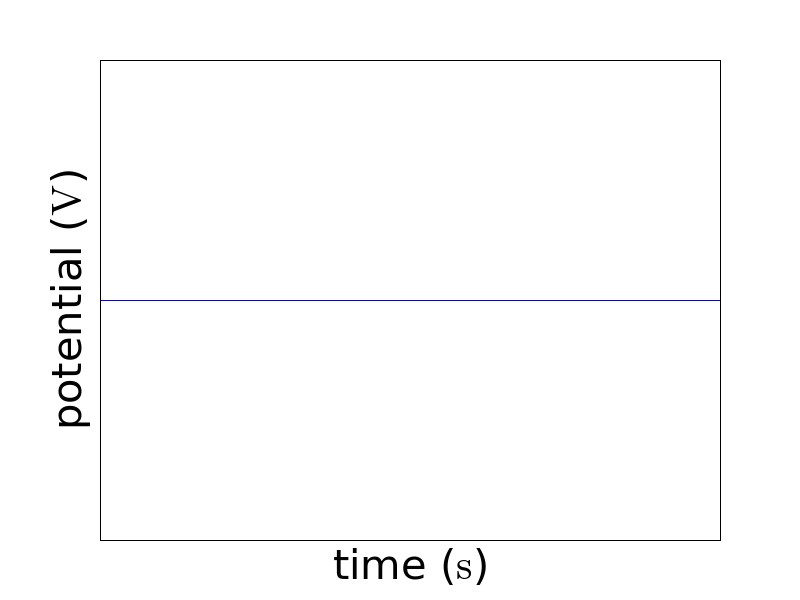
\includegraphics[width=0.3\linewidth]{figures/amperometry.png}
		\label{ec-amperometry}
	}
	\subfigure[Cyclic Voltammetry]{
		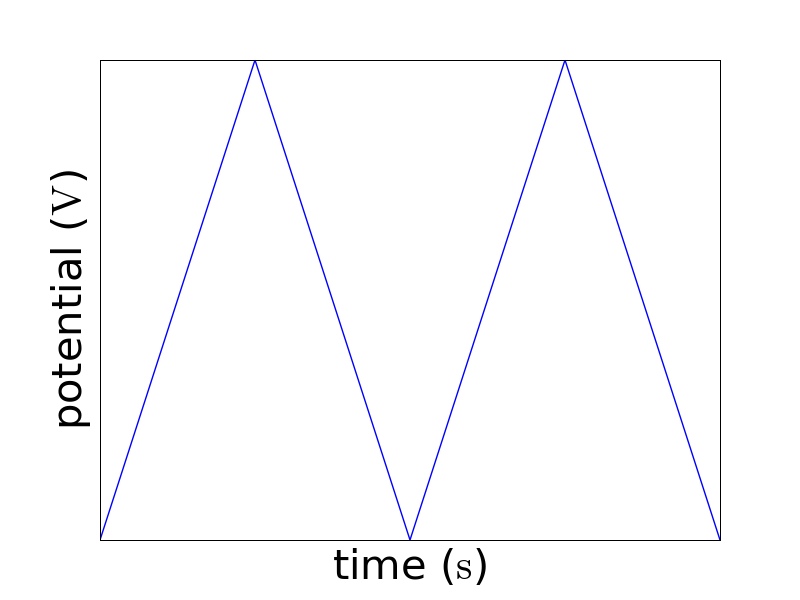
\includegraphics[width=0.3\linewidth]{figures/cv.png}
		\label{ec-cv}
	}
	\subfigure[Differential Pulse Voltammetry]{
		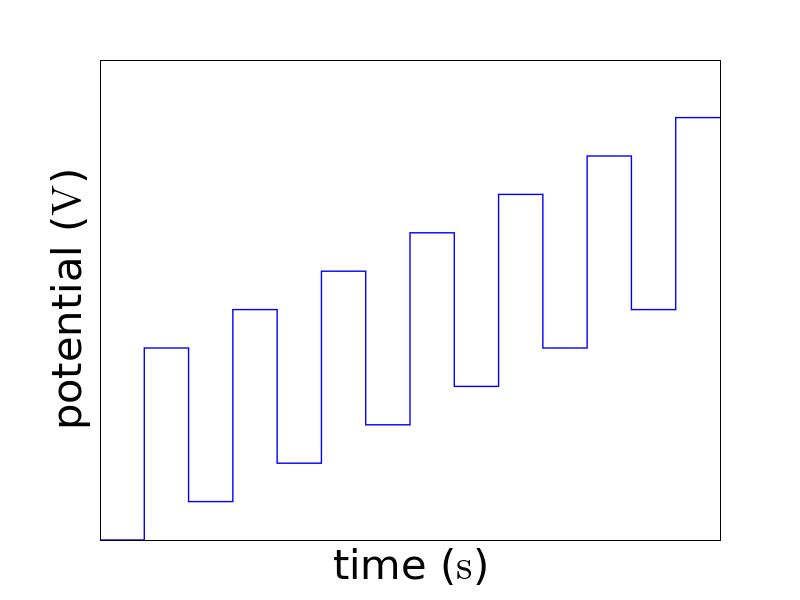
\includegraphics[width=0.3\linewidth]{figures/dpv.png}
		\label{ec-dpv}
	}
	\caption{Comparison of inputs of electrochemistry techniques}
\end{figure}

\begin{figure}
	\centering
	\subfigure[Amperometry]{
		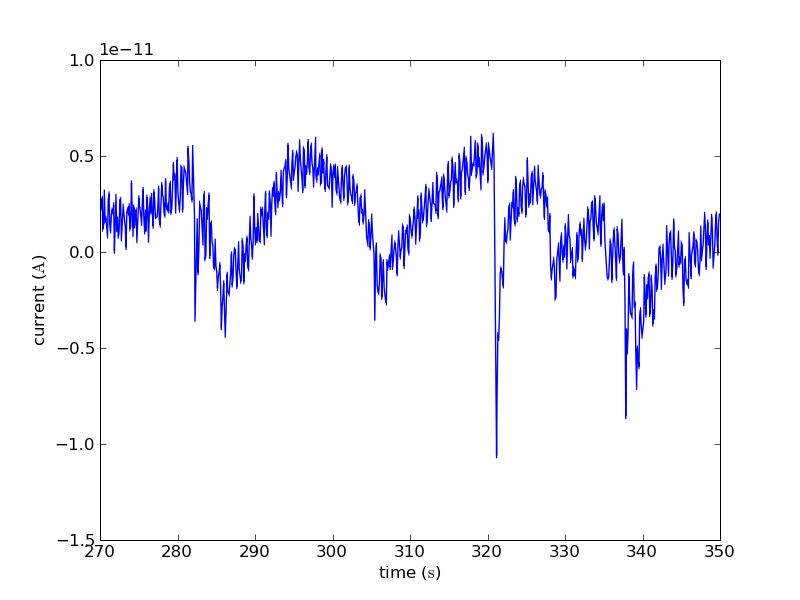
\includegraphics[width=0.3\linewidth]{figures/216.png}
		\label{ec-res-amperometry}
	}
	\subfigure[Cyclic Voltammetry]{
		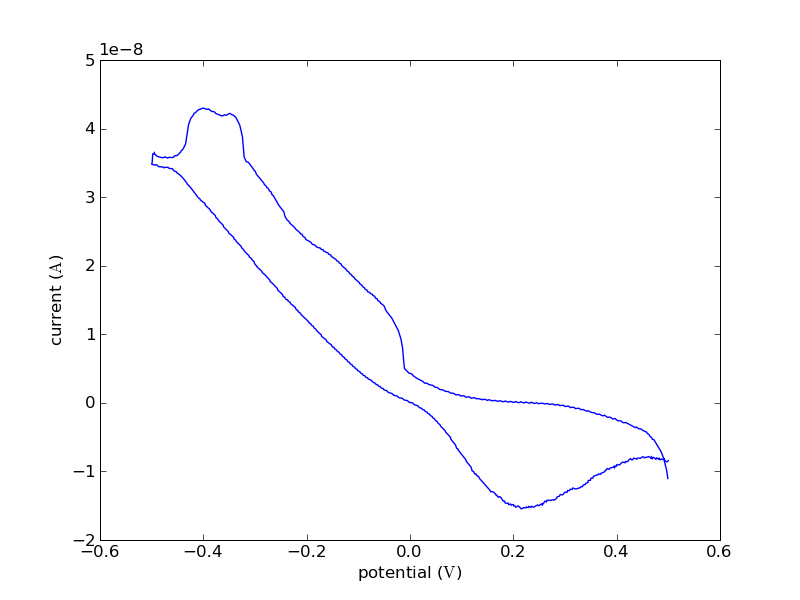
\includegraphics[width=0.3\linewidth]{figures/63.png}
		\label{ec-res-cv}
	}
	\subfigure[Differential Pulse Voltammetry]{
		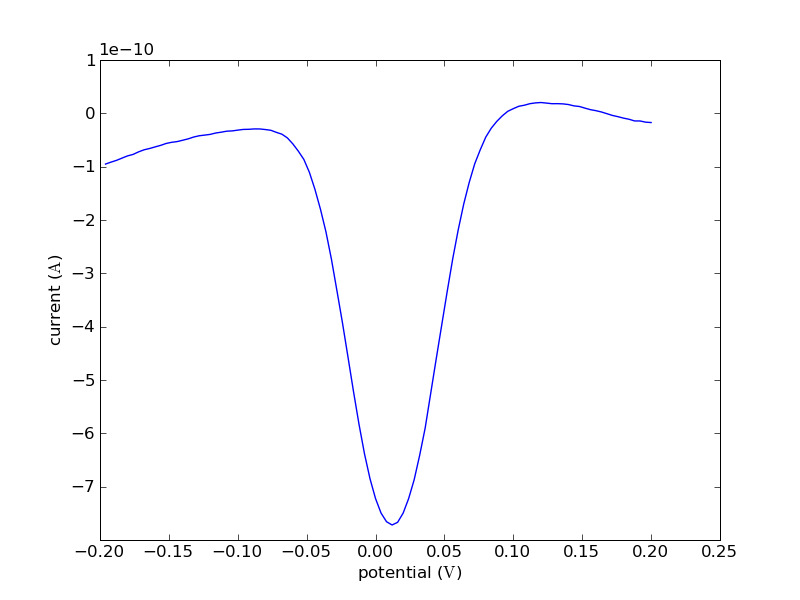
\includegraphics[width=0.3\linewidth]{figures/256.png}
		\label{ec-res-dpv}
	}
	\caption[Comparison of results of electrochemistry techniques]{Comparison of results of electrochemistry techniques. All above results were obtained by measurements on our chip.}
\end{figure}

\section{Existing Approaches}

Previous work in this field has can be divided into three fields. First, the fabrication of smaller electrodes, which are able to detect lower concentrations and can be used in integrated sensors. In 1990, Shibuki \cite{shibuki1990emd} made a $250 \mu \mathrm{m}$ electrode to detect NO, and could detect concentration changes of $1 \mu \mathrm{M}$, and reported detecting concentrations from 8--58$\mathrm{nM}$. In 1996, Bedioui et al. \cite{bedioui1996cmm} made a $50 \mu \mathrm{m}$ Pt wire with a detection limit of $170 \mu \mathrm{M}$ of nitrite (which is not low enough for biological samples). In 2002, Zhang et al. \cite{zhang2002nmn} made a $2 \mu \mathrm{m}$ electrode on a sensor chip, able to detect down to $0.3 \mathrm{nM}$ of NO. In 2002, Zhang et al. \cite{zhang2002nse} made $100 \mathrm{nm}$ electrodes with a $2 \mathrm{nM}$ detection limit. In 2003, Kim et al. \cite{kim2003img} made integrated $300 \mu \mathrm{m}$ gold electrodes able to detect down to $570 \mathrm{nM}$ of NO. In 2006, Wang et al. \cite{wang2005mcn} made a $20 \mu \mathrm{m}$ electrode able to detect down to $20 \mathrm{nM}$ of NO.

The second field is integrated potentiostats, which allows on-chip signal processing and applications to sensor arrays, where each electrode in the array has its own integrated potentiostat. In 2003, Frey et al. \cite{frey2003dip} designed and fabricated an integrated potentiostat for use in biosensor chips with output current in the 10s of $\mathrm{nA}$. In 2005, Murari et al. \cite{murari2005ipn} designed and fabricated a 16-channel integrated potentiostat with an input current range down to $8 \mathrm{pA}$. In 2007, Stanacevic et al. \cite{stanacevic2007vpa} designed a 16-channel integrated potentiostat array with an input current range down to $100 \mathrm{fA}$. In 2007, Steffan and Vrba \cite{steffan2007scp} designed an integrated potentiostat for low currents with an off-chip sensor, noting that an on-chip solution would yield better results.

The third field is electrode arrays, which allow chemical gradients to be detected. In 2001, George et al. \cite{george2001fsp} made an electrode array by screen printing, with sensors about 1 $\mathrm{mm}$ apart. In 2003, Naware et al. \cite{naware2003dam} made a $4 \times 4$ array, with square electrodes at $200 \times 200 \mu \mathrm{m}^2$. In 2005, Hafez et al. \cite{hafez2005eif} made a $2 \times 2$ array with electrodes about 3 $\mu \mathrm{m}$. In 2005, Zhang et al. \cite{zhang2005eam} made a $3 \times 3$ of nine $90 \mu \mathrm{m}$ circular electrodes, however they were all shorted together and read by on on-chip potentiostat. In 2006, Hassibi and Lee \cite{hassibi2006pmuc} made an integrated sensor array, with square electrodes at $50 \times 50 \mu \mathrm{m}^2$.

\section{Summary}

The best recent work, as described above, shows electrodes in the nanometer size, concentration detection in the nanomolar range, fully integrated potentiostats able to detect femtoamps (though at slow timescales), and integrated sensor arrays.

The above approaches show progressing work in the field of microelectrodes and integrated sensors and potentiostats. Smaller devices are being fabricated with lower detection limits. Arrays of sensors and on-chip potentiostats have been designed and shown to work. However, no thorough research has been made into shape, size, distance and configuration of integrated electrodes. The electrodes fabricated above were all either square, round, or of an unknown shape, as they were flamed or shaved down to a specific size.
